\documentclass[pdf,9pt,aspectratio=169]{beamer}
\usepackage[utf8]{inputenc}

\usepackage{DejaVuSans}
\usepackage{DejaVuSerif}
\usepackage{DejaVuSansMono}
\usepackage[T2A]{fontenc}

\usepackage[russian]{babel}

\usepackage{hyperref}
\hypersetup{unicode=true}

\usetheme{Madrid}
\usefonttheme[stillsansserifsmall]{serif}
%\usefonttheme[onlylarge]{structurebold}
\usefonttheme[onlylarge]{structureitalicserif}

\title[]{Архитектура компьютера}
\subtitle{Введение в предмет}
\author[]{Александр Рудалёв}
\institute[]{ИМИКТ САФУ}
\date[]{2016}

\usepackage{wrapfig}
\usepackage{color}
\usepackage{xcolor}

\usepackage{tikz}
\usetikzlibrary{babel}
\usetikzlibrary{shapes}

\tikzset{
  MyChar/.style={
    rectangle, rounded corners=1mm,
    minimum height=6mm,
    minimum width=4.8mm,
    very thick, draw=black!50,
    top color=white,bottom color=black!20,
    font=\ttfamily,
    text height=1.5ex,text depth=.25ex,
  },
}

\usepackage{minted}
\usemintedstyle{default} 
\newcommand{\cpil}[1]{\mintinline{python3}{#1}}

\begin{document}

\frame{\titlepage}

%%%%%%%%%%%%%%%%%%%%%%%%%%%%%%%%%%%%%%%%%%%%%%%%%%%%%%%%%%%%%%%%%%%%%%%%%%%%%%%
%%
%% Определения
%%
\begin{frame}\frametitle{Введение в предмет <<Архитектура компьютера>>}
  \begin{block}<1->{Определение}
    \textbf{Архитектура компьютера} "---  это описание его организации и принципов функционирования его структурных элементов. Включает основные устройства ЭВМ и структуру связей между ними.
  \end{block}
\end{frame}

%%%%%%%%%%%%%%%%%%%%%%%%%%%%%%%%%%%%%%%%%%%%%%%%%%%%%%%%%%%%%%%%%%%%%%%%%%%%%%%
%%
%% Вопрос
%%
\begin{frame}{Вопрос}
  \begin{columns}[T]
    \begin{column}[T]{5cm}  
      \begin{alertblock}<1->{Что это?}
        \begin{figure}
          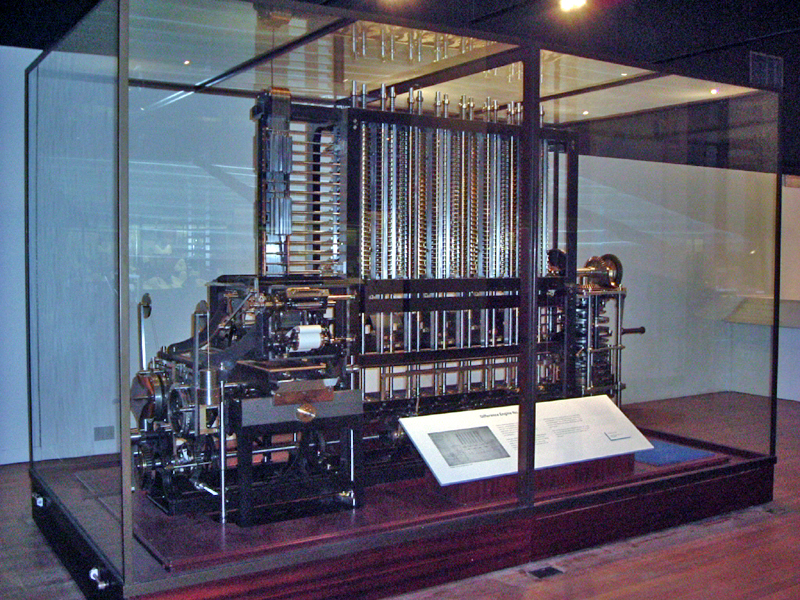
\includegraphics[width=\textwidth]{images/DifferenceEngine.jpg}
        \end{figure}
      \end{alertblock}
    \end{column}
    \begin{column}[T]{8cm}
      \begin{exampleblock}<2->{Разностная машина Чарльза Бэббиджа}
        \begin{columns}[]
          \column{2cm}
            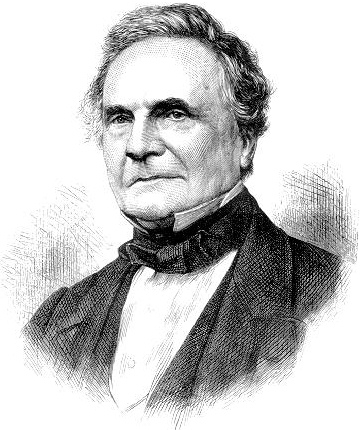
\includegraphics[width=\textwidth]{images/CharlesBabbage.jpg}
          \column{5.7cm}
              \setlength{\leftmargini}{5pt}
            \begin{itemize}
              \item До: Суммирующая машина Паскаля (1642 г.)
              \item Применение: Вычисление логарифмических таблиц.
              \item Первая статья: 1822 г.
              \item Реализация: Георг Шутц, 1854 г.
            \end{itemize}
        \end{columns}
        \begin{itemize}
          \item Прообраз для: Аналитической машины
        \end{itemize}
      \end{exampleblock}
    \end{column}
  \end{columns}
\end{frame}

\begin{frame}{Quiz}
    \begin{block}{Frage}
        With generics the compiler has more information about the 
        types of the objects, so explicit casts don't have to be used 
        and the compiler can produce type safe code.

        What implications have the generics for the runtime 
        performance of the  program which uses them?
    \end{block}

    \begin{overprint}
      \onslide<1>
      \begin{itemize}
      \item With the generics the compiler can optimize the code for 
        used types. This and the omission of the casts are the 
        reasons why the code compiled with the generics is 
        \textbf{quicker} than the one compiled without.
      \item The usage of generics has \textbf{no implications} for 
        the runtime performance of the compiled programs.
      \item The improved flexibility and type safety means that the 
        compiler has to generate concrete implementation from 
        the generic template for each used type. This means 
        that applications start \textbf{a bit slower}.
      \end{itemize}
      \onslide<2>
      The Java Virtual Machine and the copiled byte code are Generics 
      agnostic. The comiled byte code does not differ from byte code 
      compiled from sources which don't use the generics.
      So using the generics has \textbf{no impact} on the runtime 
      performance of compiled Java code.
    \end{overprint}

  \end{frame}
  \end{document}

